\chapter{Change-based Model Persistence}
This chapter presents an approach for change-based model 
persistence, as opposed to state-based model persistence,
that can facilitate high-performance incremental model processing 
(e.g., validation, transformation,
model differencing and conflict detection) by minimising the cost 
of change identification when models evolve. 
This chapter illustrates a prototype that implements the proposed
approach on top of the Eclipse Modelling Framework.

\section{Introduction}
\label{Introduction}
To reap the benefits of Model-Based Software Engineering in the context 
of large and complex systems, the ability to process large models 
in an incremental fashion as they evolve is essential. 
Current incremental model processing techniques 
(Section \ref{sec:identifying_changes_in models}) only deliver limited 
performance benefits due to slow and imprecise model change detection 
capabilities or are limited to a single-developer environment;
not realistic for real-world software development projects.
The research introduced in this paper aims at enabling flexible 
and high-performance incremental model processing through 
change-based model persistence. That is, instead of persisting snapshots 
of the state of models, this research proposes persisting models on their change history. 
The proposed approach has the potential to 
deliver step-change performance benefits in incremental model processing, 
faster model differencing and conflict detection, 
as well as a wide range of other benefits and novel capabilities.

The rest of this chapter is structured as follows. 
Section \ref{sec:running_example_1} 
present the introduction to the running example used throughout this thesis. 
Section \ref{sec:the_key_challenge_of_ _incrementality} 
reviews the key-challenge of incrementality in Model-based Software Engineering (MBSE). 
Section \ref{sec:proposed_approach} overviews our proposed approach 
and Section \ref{sec:prototype_implementation} discusses our prototype 
implementation on top of the Eclipse Modelling Framework. 
The potential benefits and novel capabilities, as well as the challenges 
of change-based model persistence, are presented in 
Sect. \ref{sec:benefits_and_novel_capabilities} and 
Sect. \ref{sec:challenges_and_future_works} respectively. 
Section \ref{sec:evaluation_strategy} presents our evaluation strategy 
and Sect. \ref{sec:conclusions} concludes this paper.

\section{Running Example: Episode 1}
\label{sec:running_example_1}
In this section, I introduce a running example to explain the key-concept of incrementality and how change-based model persistence addresses it. The running example will develops throughout this thesis as I introduce new concepts, such as presenting related work in the literature review, explaining the proposed approaches to address the slow loading of change-based models, and discussing how change-based model persistence can be exploited to optimise model differencing and conflict detection.

Let's say that there is a project to develop a simplified class diagram model of a Role Playing Game (RPG). Jane, as the technical leader, set up the initial model (Fig. \ref{fig:class_diagram_origin}). She then assigned this work to Bob and Alice. Both of them checked out this project and made some modification to the model producing the models in Figures \ref{fig:class_diagram_left} and \ref{fig:class_diagram_right} respectively.

\begin{figure}[ht]
    \begin{tabular}{l|c|r}
        \begin{subfigure}[t]{0.31\linewidth}
            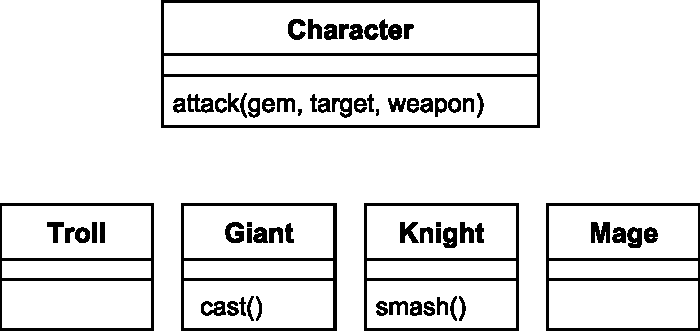
\includegraphics[width=\linewidth]{class_diagram_origin}
            \caption{original version (Jane's version)}
            \label{fig:class_diagram_origin}
        \end{subfigure}
        &
        \begin{subfigure}[t]{0.31\linewidth}
            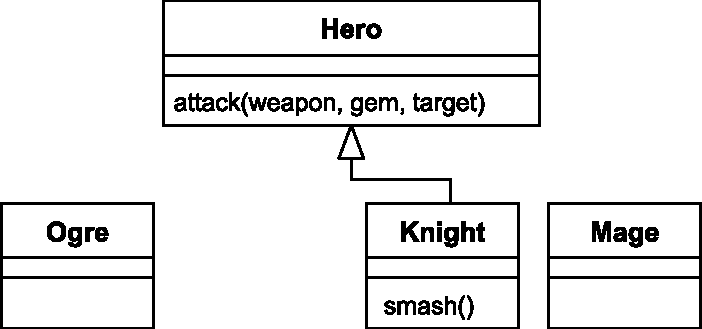
\includegraphics[width=\linewidth]{class_diagram_left}
            \caption{left version (Bob's version)}
            \label{fig:class_diagram_left}
        \end{subfigure}
        &
        \begin{subfigure}[t]{0.31\linewidth}
            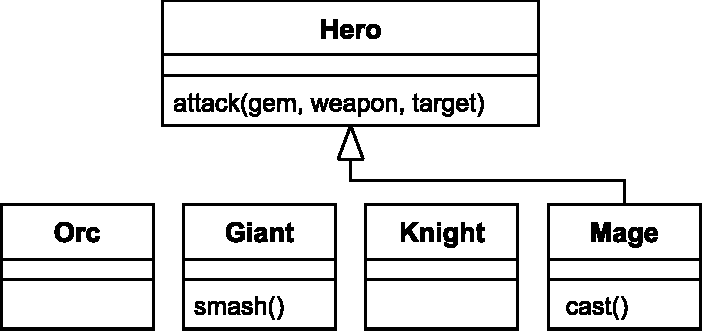
\includegraphics[width=\linewidth]{class_diagram_right}
            \caption{right version (Alice's version)}
            \label{fig:class_diagram_right}
        \end{subfigure}
    \end{tabular}
    \caption{Three class diagrams of a Role Playing Game.}
    \label{fig:class_diagram_rpg}
\end{figure}

\begin{lstlisting}[style=xmi,caption={State-based representation of the model of Figure \ref{fig:class_diagram_origin} in (simplified) XMI.},label=lst:xmimodel]
<uml:Model>
  <packagedElement type=Class id="character" name="Character">
    <operation id="attack" name="attack">
      <parameter id="gem" name="gem"/>
      <parameter id="target" name="target"/>
      <parameter id="weapon" name="weapon"/>
    </operation>
  </packagedElement>
  <packagedElement type=Class id="troll" name="Troll"/>
  <packagedElement type=Class id="giant" name="Giant">
    <operation id="cast" name="cast"/>
  </packagedElement>
  <packagedElement type=Class id="knight" name="Knight">
    <operation id="smash" name="smash"/>
  </packagedElement>
  <packagedElement type=Class id="mage" name="Mage"/>
</uml:Model>
\end{lstlisting}

\section{The Key-Challenge of Incrementality}
\label{sec:the_key_challenge_of_ _incrementality}
To illustrate the key-challenge of incrementality, I use the example in Fig. \ref{fig:class_diagram_rpg}. Let's say that after every modification to the model in Fig. \ref{fig:class_diagram_origin}, the model needs to be:

\begin{itemize}
    \item Validated against a naming convention that the name of a class should start with an uppercase.
    \item Transformed into a number of documentation files through a model-to-text transformation. Each class should have a documentation file.
\end{itemize}

Models in Figures \ref{fig:class_diagram_origin} and \ref{fig:class_diagram_left} are two consecutive versions. When the validation constraint is evaluated against the first version of the model (Fig. \ref{fig:class_diagram_origin}), it verifies that all the classes' names starts with a uppercase, and the model-to-text transformation then produces four documentation files that correspond to the classes in the model. In the sequel, in Fig. \ref{fig:class_diagram_left}, the model is updated by Bob. He applies several changes, such as renaming class \textsf{Character} to \textsf{Hero} and class \textsf{Troll} to \textsf{Ogre} and deleting class \textsf{Giant}.

A non-incremental model validation engine would treat the model of 
Fig. \ref{fig:class_diagram_left} as if it was a new model and would evaluate 
the constraint above against every class in the model. 
An incremental model validation engine, on the other hand, would identify 
that the previously established satisfaction of the constraint for classes 
\textsf{Knight} and \textsf{Mage} cannot have been possibly compromised by the changes made, and would only re-evaluate the constraint for classes \textsf{Character} and \textsf{Troll} (class \textsf{Giant} is deleted so it is not evaluated). 

Similarly, a non-incremental model-to-text transformation would generate 
and overwrite all documentation files. On the contrary, an 
incremental model-to-text transformation, would identify that it only needs to delete the documentation file of class \textsf{Giant} and generate documentation files for classes \textsf{Character} and \textsf{Troll} -- but not the documentation files of classes \textsf{Knight} and \textsf{Mage}, as these cannot have been affected by the changes made to the model.

While the overhead of executing transformations and validation constraints 
on small models like the one in Fig. \ref{fig:class_diagram_origin} is negligible, non-incremental execution can become a significant bottleneck for large evolving models. As stressed in Selic's seminal work \cite{selic2003pragmatics}, with reference to model-to-text transformation, ``... \textsf{this is particularly true in the latter phases of the development cycle when programmers make many small changes as they fine-tune the system. To keep this overhead low, it is crucial for the code generators to have sophisticated change impact analysis capabilities that minimize the amount of code regeneration}".

As demonstrated by the pioneering work of Egyed \cite{egyed2011automatically}, 
to achieve incremental re-execution of (deterministic) queries on 
structured models, an execution engine needs to:

\begin{enumerate}
    \item Record model element property accesses during the initial execution of the queries;
    \item Identify new and deleted elements and modified model element properties in the new version of the model;
    \item Combine the information collected in the steps above to identify the subset of (potentially) affected rules/queries/templates that need to be re-executed.
\end{enumerate}

To illustrate this, we use an OCL implementation of the domain-specific constraint in List. \ref{lst:constraint}.

\begin{lstlisting}[style=ocl,caption={OCL constraint requiring that a class should start with an uppercase.},label=lst:constraint]
context Class
inv UpperCase: self.name->subtring(1, 1) == self.name->subtring(1, 1)->toUpper()
\end{lstlisting}

\begin{table}[ht]
    \centering
    \caption{Property-access trace of the evaluation of the constraint in List. \ref{lst:constraint} on the model of Fig. \ref{fig:class_diagram_origin}.}
    \begin{tabular}{p{4cm} p{2.1cm} p{2cm} p{2.1cm}}
        \hline 
        \textbf{Constraint} & \textbf{Context} & \textbf{Accessed Element} & \textbf{Accessed Property} \\ 
        \hline 
        \textsf{Class.UpperCase}  & \textsf{character} & \textsf{character} & \textsf{name} \\ 
        \textsf{Class.UpperCase}  & \textsf{troll} & \textsf{troll} & \textsf{name} \\ 
        \textsf{Class.UpperCase}  & \textsf{giant} & \textsf{giant} & \textsf{name} \\ 
        \textsf{Class.UpperCase}  & \textsf{knight} & \textsf{knight} & \textsf{name} \\
        \textsf{Class.UpperCase}  & \textsf{mage} & \textsf{mage} & \textsf{name} \\
        \hline 
    \end{tabular} 
    \label{tab:property_access_trace}
\end{table}

During the initial evaluation of the constraint on the model of Fig. \ref{fig:class_diagram_origin}, an incremental OCL engine would compute the property access trace displayed in Table \ref{tab:property_access_trace} as a side-product. Now, when the model is updated (Fig. \ref{fig:class_diagram_left}), the execution engine can identify that:

\begin{itemize}
    \item There is an element deleted in the model (class \textsf{Giant}) for which the constraint is not necessary to be evaluated;
    \item The value of property \textsf{name} of classes \textsf{Character} and \textsf{Troll} have changed, and as such, the constrain needs to be re-evaluated on this elements.
\end{itemize}

Egyed has shown that the property-access recording approach is applicable to queries of arbitrary complexity, 
as long as they are deterministic. More recent work has shown that variants of this approach can be used to 
achieve incrementality in a wide range of model processing operations, including model-to-model 
transformation \cite{jouault2010towards}, model-to-text transformation \cite{DBLP:conf/ecmdafa/OgunyomiRK15}, 
model validation, and pattern matching \cite{DBLP:conf/ecmdafa/RathHV12}---as long as changes to models can be 
precisely identified (step 2 in the list above).

\section{Identifying Changes in Models}
\label{sec:identifying_changes_in models}
There are two approaches in the literature for identifying changes in models in order to enable incremental re-execution of model processing operations.

\textbf{Notifications}. In this approach, the incremental execution engine needs to hook into the notification facilities provided by the modelling tool through which the developer edits the model, so that the engine can directly receive notifications as soon as changes happen (e.g. a class has been deleted (class \textsf{Giant}), the name property of class \textsf{Troll} has been changed to ``Ogre"). This is an approach taken by the IncQuery incremental pattern matching framework \cite{DBLP:conf/ecmdafa/RathHV12} and the ReactiveATL incremental model-to-model transformation engine \cite{DBLP:conf/ecmdafa/OgunyomiRK15}. The main advantage of this approach is that precise and fine-grained change notifications are provided for free by the modelling tool (and thus do not need to be computed by the execution engine---which as discussed below can be expensive and inefficient). On the downside, this approach is a poor fit for collaborative development settings where modelling and automated model processing activities are performed by different members of the team.

\textbf{Model Differencing}. This approach eliminates the coupling between modelling tools and incremental execution engines. Instead of depending on live notifications, in this approach the developer in charge of automated model processing, needs to have access to a copy of the last version of the model that the model processing program (e.g. the model-to-text transformation) was executed upon, so that it can be compared against the current version of the model (e.g. using a model-differencing framework such as SiDiff \cite{Treude2007SiDiff} or EMF Compare \cite{eclipse2017compare} and the delta can be computed on demand. The main advantage of this approach is that it works well in a collaborative development environment where typically developers have distinct roles and responsibilities. On the downside, model comparison and differencing are computationally expensive and memory-greedy (both versions of the model need to be loaded into memory before they can be compared), thus largely undermining the time and resource saving potentials of incremental re-execution.

In summary, incremental model processing currently delivers significant performance benefits only in a single-developer environment where the modeller is also responsible for performing all the (incremental) model processing operations. As a result, in collaborative development environments, developers need to either forgo incremental model processing altogether or to work around this limitation by manually steering model processing programs to process only subsets of their models, which is cumbersome and error prone.

\section{Proposed Approach}
\label{sec:proposed_approach}
The ambition of this research is to enable high-performance incremental model management in collaborative software development environments by challenging one of the fundamental assumptions of contemporary modelling frameworks and tools: as opposed to persisting snapshots of the state of models (which is what virtually all modelling tools and frameworks currently do), this work proposes turning models inside out and persisting their change history instead.

\begin{lstlisting}[style=xml,caption={Change-based representation of the model of Figure \ref{fig:modified_chart}.},label=lst:cbpmodel]
session "Jane-01"
create character type Class
set character.name to "Character" 
create attack type Operation
set attack.name to "attack" 
add attack to character.operations at 0
create gem type Parameter
set gem.name to "gem" 
add gem to attack.parameters at 0
create target type Parameter
set target.name to "target" 
add target to attack.parameters at 1
create weapon type Parameter
set weapon.name to "weapon" 
add weapon to attack.parameters at 2
create troll type Class
set troll.name to "Troll" 
create giant type class
set giant.name to "Giant"
create cast type Operation
set cast.name to "smash"
add cast to giant.operations at 0
create knight type Class
set knight.name to "Knight"
create smash type Operation
set smash.name to "smash"
add smash to knight.operations at 0
create mage type Class
set mage.name to "Mage" 
session "Bob-01"
create leftGen type Generalization
set leftGen.general to character
set troll.generalization to leftGen
set character.name from "Character" to "Hero"
remove leftGen from troll.generalization composite r1
set knight.generalization to leftGen composite r1
move target in attack.parameters from 1 to 2
unset cast.name from "cast" to null composite r2
remove cast from giant.operations at 0 composite r2
delete cast composite r2
unset giant.name from "Giant" to null composite r2
delete giant comp r2
set troll.name from "Troll" to "Ogre"
\end{lstlisting}

To illustrate the proposed approach, List. \ref{lst:xmimodel} shows a state-based representation of the model of Fig. \ref{fig:modified_chart} in (simplified) XMI, and List. \ref{lst:cbpmodel} shows the proposed equivalent change-based representation of the same model. Instead of a snapshot of the state of the model, the representation of List. \ref{lst:cbpmodel} captures the complete sequence of change events (create/set/add/remove/delete) that were performed on the model since its creation, organised in editing sessions (2 editing sessions in the case of this model). Replaying these changes produces the same state as the one captured in List. \ref{lst:xmimodel}, so the proposed representation carries at least as much information as the state-based representation.

Such a representation is particularly suitable for incremental model processing. For example, if the model-to-text transformation discussed above ``remembers" that in its previous invocation it had processed up to editing session \textsf{s1} of the model, it can readily identify the changes that have been made to the model since then (i.e. in session \textsf{s2} –- lines 15-20) instead of having to rediscover them through (expensive) state-based model differencing.

\section{Prototype Implementation}
\label{sec:prototype_implementation}
This work has implemented a prototype\footnote{The prototype is available under \url{https://github.com/epsilonlabs/emf-cbp}.} of the change-based model persistence format using the notification facilities provided by the Eclipse Modelling Framework. In the implementation, the prototype uses a subclass of EMF's \textsf{EContentAdapter} (\textsf{ChangeEventAdapter}) to receive and record \textsf{Notification} events produced by the framework for every model-element level change.

\begin{figure}[th]
    \centering
    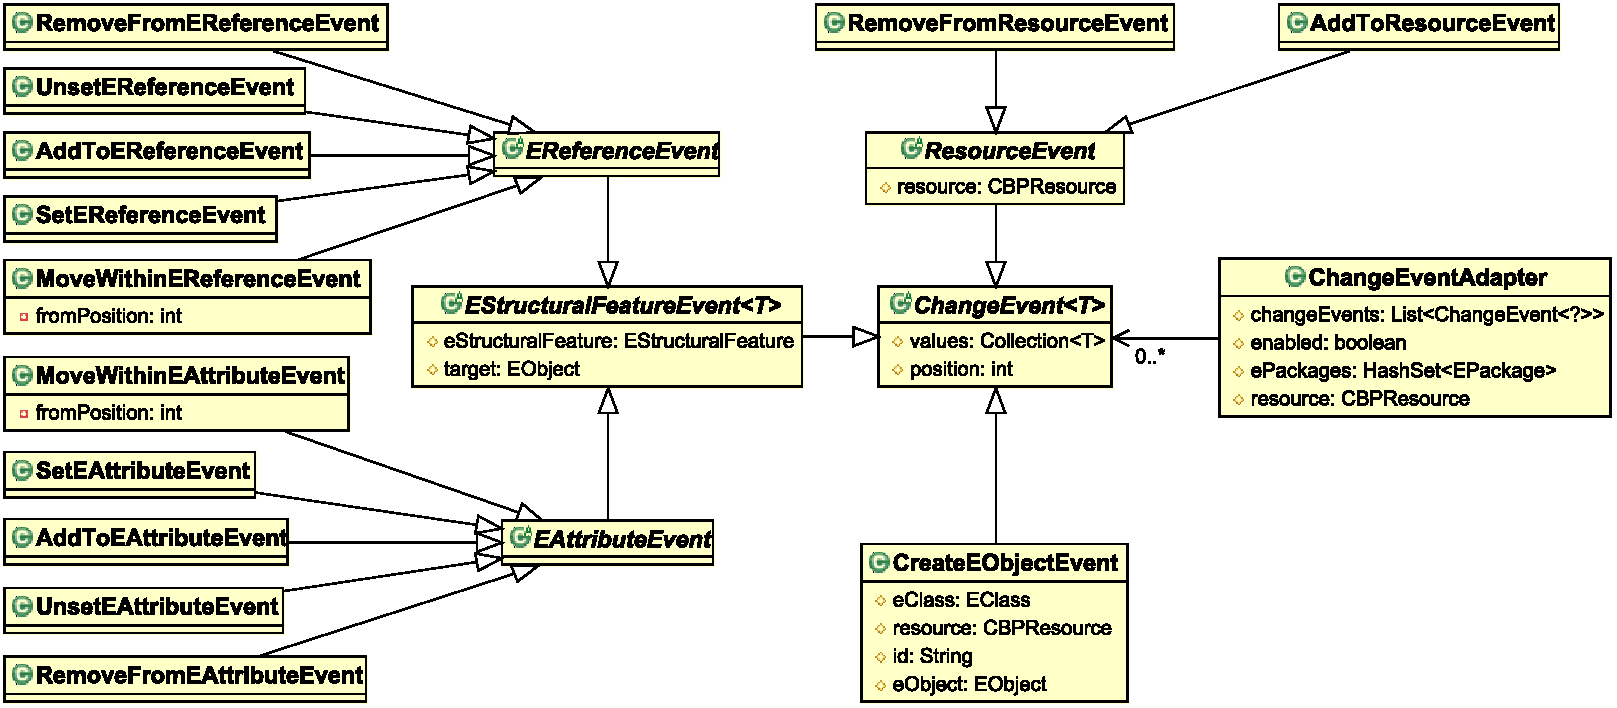
\includegraphics[width=\linewidth]{events}
    \caption{Event classes to represent changes of models.}
    \label{fig:events}
\end{figure}

Since not all change events are relevant to change-based persistence (e.g. EMF also produces change notifications when listeners/adapted are added/removed from the model), this work has defined a set of event classes to represent events of interest. The event classes are depicted in Fig. \ref{fig:events} as subclasses of the \textsf{ChangeEvent} abstract class.

The \textsf{ChangeEvent} class has a mutli-valued \textsf{values} attribute which can accommodate both single-valued (e.g. set/add) or mutli-valued events (e.g. addAll/removeAll). \textsf{ChangeEvent} can also accommodate different types of values, such as \textsf{EObject}s for \textsf{EReferenceEvents}, and primitive values (e.g. Integer, String) for \textsf{EAttributeEvents}. The \textsf{ChangeEvent} class also has a position attribute to hold the  index of an \textsf{EObject} or a literal when they are added to a \textsf{Resource}, \textsf{EReference}, or \textsf{EAttribute} with multiple values (Lst. \ref{lst:cbpmodel}, line 3, 6, 9, 12, 14, 17, 20). 

Every time an \textsf{EObject} is added to the model, a \textsf{CreateEObjectEvent} and an \textsf{AddToResourceEvent} are recorded (lines 2-3, 5-6, 8-9, and 16-17 in Lst. \ref{lst:cbpmodel}). When an EObject is deleted, or moved to a containment \textsf{EReference} deeper in the model (Lst. \ref{lst:cbpmodel}, line 12, 14, 20), a \textsf{RemoveFromResourceEvent} (Lst. \ref{lst:cbpmodel}, line 11, 13, 19) is recorded.

The \textsf{ChangeEventAdapter} receives EMF change notifications in its \textsf{notifyChanged()} method and filters and transforms them into appropriate change events. As an example of how notifications are filtered and transformed, Listing \ref{lst:javacode} shows how the prototype handles \textsf{Notification.UNSET} events based on the type of the changed feature i.e. an \textsf{UnsetEAttributeEvent} is instantiated if the feature of the notifier is an \textsf{EAttribute}, or an \textsf{UnsetEReferenceEvent}  is created if the notifier is an \textsf{EReference}. The transformed instances are then stored into a list of events in \textsf{ChangeEventAdapter} (\textsf{changeEvents}) for persistence. 

\begin{lstlisting}[style=java,caption={Simplified Java code to handle notification events.},label=lst:javacode]
public class ChangeEventAdapter extends EContentAdapter {
...
@override
public void notifyChanged(Notification n) {
    ...
    switch (n.getEventType()) {
    ... // other events
    case Notification.UNSET: {
        if (n.getNotifier() instanceof EObject) {
            EStructuralFeature feature = (EStructuralFeature) n.getFeature();
            if (feature instanceof EAttribute) {
                event = new UnsetEAttributeEvent();
            } else if (feature instanceof EReference) {
                event = new UnsetEReferenceEvent();
            }
        } break;
    } 
    ... // other events
\end{lstlisting}	

To integrate seamlessly with the EMF framework and to eventually support multiple concrete change-based serialisation formats (e.g. XML-formatted representation for readability and binary for performance/size), the prototype implemented \textsf{CBPResource} abstract class, that extends EMF's built-in \textsf{ResourceImpl} class. The role of the abstract class is to encapsulate all change recording functionality while the role of its concrete subclasses is to implement serialisation and de-serialisation. For example, \textsf{CBPXMLResourceImpl} persists changes in a line-based format where every change is serialised as a single-line XML document. In this way, when a model changes, the prototype can append the new changes to the end of the model file without needing to serialise the entire model again. The prototype has also implemented a \textsf{CBPXMLResourceFactory} class that extends EMF's \textsf{ResourceFactoryImpl}, as the factory class for change-based models. Figure \ref{fig:resources} shows the relationships between these classes.

\begin{figure}[th]
    \centering
    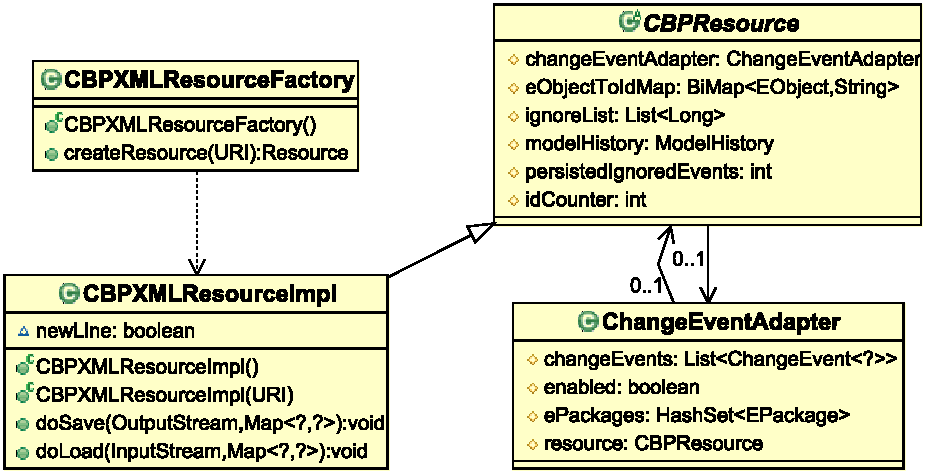
\includegraphics[width=0.75\linewidth]{resources}
    \caption{Factory, resources, and ChangeEventAdapter classes.}
    \label{fig:resources}
\end{figure}

\section{Benefits and Novel Capabilities}
\label{sec:benefits_and_novel_capabilities}
Beyond facilitating incremental processing, the proposed representation 
also has the potential to deliver a wide range of benefits and 
novel capabilities, compared to the currently prevalent 
state-based representations, some of which are discussed below.

\begin{itemize}
    \item With appropriate tool support, modellers will be able to ``replay" (part of) the change history of a model (e.g. to understand design decisions made by other developers, for training purposes). In state-based approaches, this can be partly achieved if models are stored in a version-control repository (e.g. Git). However, the granularity would only be at the commit level.
    \item By analysing models serialised in the proposed representation, modelling language and tool vendors will be able to develop deeper insights into how modellers actually use these languages/tools in practice and utilise this information to guide the evolution of the language/tool.
    \item By attaching additional information to each session (e.g. the id of the developer, references to external documents/URLs), sequences of changes can be traced back to the developer that made them, or to requirements/bug reports that triggered them.
    \item Persisting changes to large models after an editing session will be significantly faster compared to serialising the entire state of the model, as only changes made during the session will need to be appended to the model file.
    \item The performance and precision of model comparison and merging can be substantially improved, particularly for large models with shared editing histories.
\end{itemize}

\section{Challenges}
\label{sec:challenges}
The proposed approach also comes with a number of challenges that this research will need to overcome, such as loading overhead and fast-growing model files. However, due to limitation of time, this work only addresses the loading overhead while the fast-growing model files can be set as another topic for future work.  

While, as discussed above, persisting changes to large models is expected to be much faster and resource-efficient compared to state-based approaches, loading models into memory by naively replaying the entire change history is expected to have a significant overhead. To address this challenge, this work has developed two solutions that reduces the cost of change-based model loading, firstly, by recording and ignoring events -- events that are later overridden or cancelled out by other events -- and, secondly, by proposing a hybrid model persistence format which models are loaded from stated-based persistence but changes are persisted into both change-based and state-based representation. 

For the fast-growing model files challenge, persisting models in a change-based format means that model files will keep growing in size during their evolution significantly faster than their state-based counterparts. To address this challenge, one can proposes sound change-compression operations (e.g. remove older/unused information) that can be used to reduce the size of a model in a controlled way or develops a compact textual format that will minimise the amount of space required to record a change (a textual line-separated format is desirable to maintain compatibility with file-based version control systems).  

\section{Conclusions}
\label{sec:conclusions_2}
Through persisting models' change history, this research aims at enabling high-performance incremental model processing in collaborative development settings. The proposed approach also has the potential to enable model analytics, more fine-grained tracing, and to improve the precision and performance of model comparison and merging. A prototype implementation of a change-based persistence format has been presented and the main envisioned challenges have been listed. 